
\section{Oriented percolation}

\begin{frame}
	\frametitle{Oriented percolation as an example of  bootstrap percolation}
	
\begin{itemize}
\item Oriented percolation (OP) is one of the simplest subcritical BP model.
\item It is a BP model with one-family rule $\mathcal{U} = \{U\} = \{\{-1, 1\}, \{1, 1\}\}$
\item Some of the well-known results in the field are reviewed in Durrett's article \footnote{R. \textsc{Durret}, \emph{Oriented Percolation in Two DImensions}, The Annals of Probability}
\item We will follow this article to introduce some non-trivial results about OP
\end{itemize}

\begin{alertblock}{Remark}
	In the article of Durrett bond percolation is considered rather than site. However, by one simple trick one can show that in the case of OP the two are equivalent.
\end{alertblock}

\end{frame}

\begin{frame}
	there will be an image with the trick
\end{frame}

\begin{frame}
	\frametitle{Edge speed}
	\begin{itemize}
		\item We remind that the parameter of OP - $p = 1 - q$ stands for the intensity of \textbf{healthy} sites
		\item We let $p_{c}^{OP}$ be the critical probability for OP
		\item We say that $x \rightarrow y$  if there exist $x_{0} = x, x_{1}, \ldots, x_{n} = y$ such that $x_{i} - x_{i - 1} \in \mathcal{U}$ and $x_{i}$ open for $0 < i \leq n$, i.e. there exists an OP path between x and y.
		\item We are naturally interested in the event $\{0 \rightarrow \infty \} = \{ \cap_{i = 1}^{\infty} L_{i} \neq \emptyset \}$, where $L_{n} = \{x: (0, 0) \rightarrow (x, n) \}$ - the set of sites on the height n connected to 0.
		\item Notice that saying that $0 \rightarrow \infty$ is equivalent to saying that 0 is not infected in the BP model (duality BP - OP).
	\end{itemize}
\end{frame}
	
\begin{frame}
	\frametitle{Edge Speed}
	\begin{itemize}
		\item We denotel $r_{n} = \sup \{x \in \mathbb{Z}, \exists y \leq 0, (y, 0) \rightarrow (x, n)\}$ - the rightmost edge with the convention $\sup \{\emptyset\} = - \infty$
		\item This definition may seem a bit artificial at first glance (why would we look at $(y, 0) \rightarrow (x, n)$ for some $y \leq 0$ rather than $(0, 0) \rightarrow (x, n)$)?
	\end{itemize}
	\begin{block}{Property}
		Provided that $L_{n} \neq \emptyset$, we have r$_{n} = \sup L_{n} = \sup \{x: (0, 0) \rightarrow (x, n) \} $
	\end{block}
	\begin{block}{Proof by a picture}
		\begin{figure}
			\caption{Taken from Durret's review}
			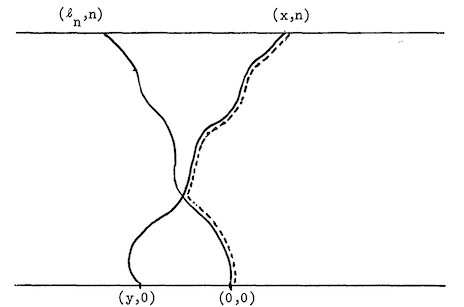
\includegraphics[height = 3cm]{image_edge_speed}
			\centering
		\end{figure}
	\end{block}
\end{frame}

\begin{frame}
	\frametitle{Edge speed}
	\begin{itemize}
		\item We now want to quantify the asymptotic behaviour of $\frac{r_{n}}{n}$
	\end{itemize}
	\begin{block}{Theorem - definition}
		There exists a function $\alpha: [0, 1] \rightarrow [- \infty, 1]$ called edge speed with the following property:
		$$
			\frac{r_{n}}{n} \rightarrow \alpha (p) = \inf_{n} \mathbb{E}_{p}[r_{n}/n]
		$$
		Moreover, we have that $\alpha$ is continuous and strictly increasing on $[p_{c}^{OP}, 1]$ with $\alpha(p_{c}^{OP}) = 0, \alpha(1) = 1$ and $\alpha(p) = -\infty$ for $p < p_{c}^{OP}$.
	\end{block}
	\begin{itemize}
		\item Intuitively edge speed tells us how far the rightmost path (starting from height 0 and to the left of the origin) is expected to go.
		\item Edge speed has the following "criticality" properties which we state without proof
	\end{itemize}

\end{frame}

\begin{frame}
	\frametitle{Properties of edge speed}
	\begin{block}{Property 1}
		For $p > p_{c}^{OP}$ (above criticality for OP) and $\alpha_{0} < \alpha(p)$ with positive probability there exists an infinite OP path $((a_{i}, i))_{i \in \mathcal{N}}$ with $a_{0} = 0$ and $\inf_{n} \frac{a_{n}}{n} \geq \alpha_{0}$. Intuitively this means that we have chances to get an infinite path that goes sufficiently far (but below edge speed) to the right.
	\end{block}

	\begin{block}{Property 2}
		For $\alpha_{0} > \alpha(p)$, for some $\gamma > 0$ we have 
		$$
			\mathbb{P}_{p}(r_{n} \geq \alpha_{0} n) \leq e^{-\gamma n}
		$$
		This exponential decay shows that it is unlikely to find a path that goes too far (further than edge speed) to the right.	
	\end{block}
\end{frame}

\begin{frame}
	\frametitle{Critical densities of OP}
	\begin{itemize}
		\item We let $\psi (u) = 1 - \alpha^{-1}(|tan(u)|)$, where $\alpha^{-1}$ is the inverse of the edge speed function $\alpha$.
		\item The following theorem expresses the critical density of OP depending on the direction $u$ which is parametrized by the angle it makes with the origin: $u \in [- \pi, \pi]$.
	\end{itemize}
	\begin{block}{Theorem}
		The critical densities of the BP percolation with $\mathcal{U} = \{(1, 1,) (-1, 1)\}$ (dual to OP) are given by
		\begin{equation}
			d_{u}(\mathcal{U})= \begin{cases}0, & u \in[-3 \pi / 4,-\pi / 4] \\ 1-p_{\mathrm{c}}^{\mathrm{OP}}=q_{\mathrm{c}}, & u \in[0, \pi] \\ \psi(u), & \text { otherwise }\end{cases}
		\end{equation}
	\end{block}
\end{frame}

\begin{frame}
	\frametitle{Outline of the proof}
	\begin{itemize}
		\item If $u \in (-3\pi/4, -\pi/4)$, we have $[\mathbb{H}_{u}] = \mathbb{Z}^{2}$ (the directions are unstable), so in this case $d_{u} = 0$
		\item By symmetry it suffices to treat $u \in [-\pi/4, \pi/2]$
		\item The critical density $d_{u}$ can be thought as the value $\tilde{q}$ above which a.s there is no oriented infinite path from the origin which does not pass by $\mathbb{H}_{u}$
		\item It suffices then to show that below $\tilde{q}$ there is such an infinite path with positive probability and above it does not exist a.s.
		\item For $q < q'$ one can prove that it in order not to pass by $\mathbb{H}_{u}$ it suffices to go to the right with the speed below edge speed which is possible (with positive probability) by the property 2
		\item Conversely, for $q > \tilde{q}$, we would have to walk to the right above edge speed to get around $\mathbb{H}_{u}$ which is not possible (exponential decay) 
	\end{itemize}
\end{frame}

\begin{frame}
	\frametitle {Open questions and conjectures about OP}
	\begin{itemize}
		\item We remind that $q_{c}=\inf \left\{q \in[0,1], \mathbb{P}_{q}\left([A]=\mathbb{Z}^{2}\right)=1\right\}$, whereas $\tilde{q}_{c}=\inf \left\{q \in[0,1], \sum_{n} n \theta_{n}(q)<\infty\right\}$
	\end{itemize}
	\begin{block}{Conjecture}
		For all BP models (all update families) we have: $q_{c} = \tilde{q}_{c}$.
	\end{block}
	\begin{itemize}
		\item It would be practical to know if the complication of taking right and left limits to define the critical density $d_{u} = max(d_{u}^{+}, d_{u}^{-})$ is necessary.
	\end{itemize}
	\begin{block}{Question}
		What are the continuity properties of the function $(u, \theta) \rightarrow d_{u}^{\theta}$?
	\end{block}
\end{frame}



